%to have line numbers
%\RequirePackage{lineno}
\documentclass[10pt, letterpaper]{article}      
\usepackage[margin=.1cm,font=small,labelfont=bf]{caption}[2007/03/09]
%\usepackage{endnotes}
%\let\footnote=\endnote


\usepackage{setspace}
\usepackage{longtable}                        
\usepackage{anysize}                          
\usepackage{natbib}                           
%\bibpunct{(}{)}{,}{a}{,}{,}                   
\bibpunct{(}{)}{,}{a}{}{,}                   
\usepackage{amsmath}
\usepackage[% draft,
pdftex]{graphicx} %draft is a way to exclude figures                
%\usepackage{epstopdf}
\usepackage{hyperref}                             % For creating hyperlinks in cross references
 
% \usepackage[margins]{trackchanges}

% \note[editor]{The note}
% \annote[editor]{Text to annotate}{The note}
%    \add[editor]{Text to add}
% \remove[editor]{Text to remove}
% \change[editor]{Text to remove}{Text to add}

%TODO make it more standard before submission: \marginsize{2cm}{2cm}{1cm}{1cm}
\marginsize{1cm}{1cm}{.5cm}{.5cm}%{left}{right}{top}{bottom}   
					          % Helps LaTeX put figures where YOU want
 \renewcommand{\topfraction}{1}	                  % 90% of page top can be a float
 \renewcommand{\bottomfraction}{1}	          % 90% of page bottom can be a float
 \renewcommand{\textfraction}{0.0}	          % only 10% of page must to be text

 \usepackage{float}                               %latex will not complain to include float after float

\usepackage[table]{xcolor}                        %for table shading
\definecolor{gray90}{gray}{0.90}
\definecolor{orange}{RGB}{255,128,0}

\renewcommand\arraystretch{.9}                    %for spacing of arrays like tabular

%-------------------- my commands -----------------------------------------
\newenvironment{ig}[1]{
\begin{center}
 %\includegraphics[height=5.0in]{#1} 
 \includegraphics[height=3.3in]{#1} 
\end{center}}

 \newcommand{\cc}[1]{
\hspace{-.13in}$\bullet$\marginpar{\begin{spacing}{.6}\begin{footnotesize}\color{blue}{#1}\end{footnotesize}\end{spacing}}
\hspace{-.13in} }

%-------------------- END my commands -----------------------------------------



%-------------------- extra options -----------------------------------------

\usepackage{pdfpages} %load after xcolor, like at the end ideally i guess and
                      %turn off epstopdf


%%%%%%%%%%%%%
% footnotes %
%%%%%%%%%%%%%

%\long\def\symbolfootnote[#1]#2{\begingroup% %these can be used to make footnote  nonnumeric asterick, dagger etc
%\def\thefootnote{\fnsymbol{footnote}}\footnote[#1]{#2}\endgroup}	%see: http://help-csli.stanford.edu/tex/latex-footnotes.shtml

%%%%%%%%%%%
% spacing %
%%%%%%%%%%%

% \abovecaptionskip: space above caption
% \belowcaptionskip: space below caption
%\oddsidemargin 0cm
%\evensidemargin 0cm

%%%%%%%%%
% style %
%%%%%%%%%

%\pagestyle{myheadings}         % Option to put page headers
                               % Needed \documentclass[a4paper,twoside]{article}
%\markboth{{\small\it Politics and Life Satisfaction }}
%{{\small\it Adam Okulicz-Kozaryn} }

%\headsep 1.5cm
% \pagestyle{empty}			% no page numbers
% \parindent  15.mm			% indent paragraph by this much
% \parskip     2.mm			% space between paragraphs
% \mathindent 20.mm			% indent math equations by this much

%%%%%%%%%%%%%%%%%%
% extra packages %
%%%%%%%%%%%%%%%%%%

\usepackage{datetime}

%\usepackage{polski}
\usepackage[utf8]{inputenc}
% \usepackage[latin1]{inputenc}
\usepackage{tikz}
\usetikzlibrary{shapes,arrows,backgrounds}


%\usepackage{color}					% For creating coloured text and background
%\usepackage{float}
\usepackage{subfig}                                     % for combined figures

\renewcommand{\ss}[1]{{\colorbox{blue}{\bf \color{white}{#1}}}}
\newcommand{\ee}[1]{\endnote{\vspace{-.10in}\begin{spacing}{1.0}{\normalsize #1}\end{spacing}\vspace{.20in}}}
\newcommand{\emd}[1]{\ExecuteMetaData[/tmp/tex]{#1}} % grab numbers  from stata

%TODO before submitting comment this out to get 'regular fornt'
\usepackage{sectsty}
\allsectionsfont{\normalfont\sffamily}
\usepackage{sectsty}
\allsectionsfont{\normalfont\sffamily}
\renewcommand\familydefault{\sfdefault}

% \usepackage[margins]{trackchanges} (LM)
\usepackage{rotating}
\usepackage{catchfilebetweentags}

\usepackage{abstract}
\renewcommand{\abstractname}{}    % clear the title
\renewcommand{\absnamepos}{empty} % originally center
%-------------------- END extra options -----------------------------------------
\date{{}\today}
\title{  % remember to have Vistula University!!
Elderly Volunteering and Well-Being in Europe. Revisting Haski (2009) \footnote{This study was funded by grant \# 2016/21/B/HS4/03058 from
  Polish National Science Foundation (Narodowe Centrum Nauki).}
}
\author{
Leszek Morawski\thanks{EMAIL: ???@???
  \hfill I thank XXX.  All mistakes are mine.} \\
{\small Vistula University}
Adam Okulicz-Kozaryn\thanks{EMAIL: adam.okulicz.kozaryn@gmail.com
  \hfill I thank XXX.  All mistakes are mine.} \\
{\small Rutgers - Camden  and Vistula University}
}

\begin{document}

%%\setpagewiselinenumbers
%\modulolinenumbers[1]
%\linenumbers

\bibliographystyle{/home/aok/papers/root/tex/ecta}
\maketitle
\vspace{-.4in}
\begin{center}

\end{center}


\begin{abstract}
\noindent
\end{abstract}
\vspace{.15in} 
\noindent{\sc XXX TODO add to ebib as keyword PAPER-CODE-NAME and tag with ebib keywords 
}
\vspace{.25in} 

\begin{spacing}{1.4} %TODO MAYBE before submission can make it like 2.0
\rowcolors{1}{white}{gray90}

%  instead \ExecuteMetaData[../out/tex]{ginipov} do \emd{ginipov}

% \begin{figure}[H]
%  \includegraphics[height=3in]{../out/gov_res_trust.pdf}\centering\label{gov_res_trust}
% \caption{woo}
% \end{figure}



%TODO !!!! have input here aok_var_des
%%%%%%%%%%%%%%%%%%%%%%%%%%%%%%%%%%%%%%%%%%%%%%%%%%%%%%%%%%%%%%%%%%%%%%%%%%%%%%

The countries' rates of volunteering among the group of 50+ are much dispersed. The published rates for a given country can differ significantly. due to different definitions of a volunteering  applied by authors and due to different datasets used. For example, according to \citet{Oecd16}the rates ranged from above 30\% in the Netherlands, Irleand, Norwey, Switzerland to around 10\% in Poland, Hungary, Greece, Portugal  if the Gallup data were used. On the other hand \citet{Oecd15}shows the rate of 2.3\% for Poland and 4.9\% for Portugal if the SHARE data were applied. Even though the levels differ among the sources the higher rates are usually in better developed countries. \\ 

Volunteering changes with age. Its popularity differs among age groups. In some european countries - e.g. the Netherlands, France,Denmark and the UK  - the volunteering rates are the highest among the group of 50+. In other countries - Norwey, Germany, Finland, Icleand,Switzerland  - the rates among elderly are higher than among the mid-age group (30-50) but they are above the rates for the group of 15-29. But there is also  a group of european countries in which people in age 50 and above are involved in the volunteering less often than the other age group. These are the Central and East European countries (CEE) - Estonia, Latvia,Poland, Czech Republic, Lithuania, Hungary - and  Southern European Countries (SEC) - Spain and Italy \citet{Oecd16}. It seemms that there is no unique relationship between age and volunteering. It is quite possible that it can have a different shape for different countries. \\  

The motives among elderly are also presumably different to those for younger people (\citet{wilson12}). We are usually focus on determinants at the individual level to explain the motivation to volunteer. Menchik and Weisbrod (1987)suggest two explanations for volunteering. They propose to treat it either as an ordinary consumption good or as an investment increasing an individual's income over time. \citet{haski09} pointed out that elderly in comparison with young people are less motivated by carrer concerns and  more by social motive and that unpaid work give a  chance to participate in the usefull activities. In the Freeman "good conscience hypothesis" (Freeman, 1997) volunteering is something that people feel morally obligated to do when asked. At macroecnomic level we may distinguish  between demand and supply factors. The demand for volunteering is mostly created by unmet demand for public goods and services. The supply depends on how people allocate their time to unpaid activities to improve her utility \citet{ziemek06}. Economic approach  suggests the relation between the degree of unsatisfactory supply of public good and services and the rates of volunteering. Inefficient markets and weak government are important determinants of popularity of volunteering in this approach. Hence, the volunteering should be more popular in less developed countries where markets are inefficient and quality of goverment is low. However, this prediction seems to be false since Hank and Stuck
(2008) and Siegrist and Wahrendorf (2009)  give robust conclussion ob the higher rates in Northern European countries and lower rates in Eastern and Southern Europe. The same pattern appears in \citet{Oecd15} that shows the rates in formal volunteering range from 57.3\% in Norway to 17.7\% in Czechia. Variation in the rates is even larger if we concentrate on the volunteering among people aged 50 and over. Then it ranges from 37.9\% in the Netherlands to as little as 3.2\% in Poland. The higher rates in better developed countries suggest a considerable role of supply factors as well ass the role of public policy in overcoming the barriers to volunteering. Among then we should mention transport difficulties, lack of information, perceptions of volunteering and lack of variety in the opportunities.  \\

The low rates among less developed countries are worrying in the times of rising the problem of ageing. One may expect that the demographic changes and financial distress in retirement sector  will touch elderly in a especially adversely way.  Quality of life of elderly has become a major social issue. Elderly are likely to experience negative events due to health deterioration, reduction of income and smaller social contact network. Volunteering may improve their QoL through engagement in a socially meaningful role. Volunteering builts up social networks and gives meaning and purpose in life (Greenfield and Marks, 2004; Prouteau and Wolff, 2008). The positive consequences of being engaged in volunteering by elderly are well known and commonly accepted. Formal volunteering reduces depressive symptoms among older and older people seem to benefit more from volunteering than younger people (Li and Ferraro, 2005; Van Willigen, 2000). \citet{jenkinson2013volunteering} surveyed forty experimental and cohort studies comparing the physical and mental health outcomes and mortality of a volunteering group to a non-volunteering group and they found that volunteering had favourable effects on depression, life satisfaction, wellbeing but not on physical health. Positive association between vounteering and subjective health was reported in for example in  \citet{borgonovi08}, \cite{anderson14}, \cite{li06}, \cite{VanWilligen00}, \citet{detollenaere17}. It is commonly agreed that helping others positive effects wellbeing of volunteering. Those engaged in such activity report higher scores for subjective well-being (\citet{haski09}, \citet{morrow2003}, \citep{thoits03}, \citep{whillans2016}). \citep{meier08} showed that volunteering led to increased life satisfaction in a longitudinal study in Germany. \citet{wilson12} in his review essay on volunteerism research  listed the benefits of volunteering for the volunteer. The list included: enchancement in mental health and protection against symptoms of mentall illness, lower levels of morbidity and mortality, socioeconomic benefits such as increase in chances of obtaining a better education and a better job. Positive effect of volunteering was also found in a study based on 30 case studies from 11 European countries (\citet{ehlers11}). It was stressed that volunteering of elderly people help them to build new relationships with other volunteers but also with those whom the helped. According to findings presented in the study volunteering helps regain a meaningful activities after some adverse events.   \\

Volunteering is beneficial for society ( \citet{Oecd15}, \cite{prouteau06}, japonka). It is often treated as a productive activity (\citet{hank09}). This is importnat since demographic changes combined with progress in health care add to increasing time while people are in relatively good health while being on retirement. This creates additional  stock of unused labor among elderly that may be effectively used with benefit for volunteer and other members of a society.  It makes   volunteering of elderly to be potentially important policy tool that may help to keep people in better health when they get older. The positive effect of volunteering has been recognized by many international organizations. In its 2001 recommendations on support for volunteering, the United Nations General Assembly identified volunteering as “an important component of any strategy aimed at . . . poverty reduction, sustainable development, health, disaster prevention and management and . . . overcoming social exclusion and discrimination” (United Nations, 2001). In 2008, the European Parliament spoke of volunteering as “[the] most sustainable form of renewable energy” and encouraged Member States and regional and local authorities to “recognise [its] value . . . in promoting social and economic cohesion” (European Parliament, 2008). The year 2011 was declared the European Year of Volunteering by the European Commission (OECD, p.202). Volunteering by elderly is important and we are expecting that it will be even more important in near future. We belive that the relation between volunteering and QoL should be studied. \\


This paper follows the discussion started in \citet{haski09}.  This exceptional empirical study was based on data collected in 2005 and 2006 in the first wave of Survey of Health, Ageing and Retirement in Europe (SHARE). It included an extensive discussion of variations in volunteering rates according to main socio-economic variables as age, gender and employment status among people aged 50 or more in 12 Western and Southern European countries. As in the other studies it founded  the highest rates of voluteering among elderly in Northern Europe and the lowest rates in Southern Europe. Apart from the confrimation of many previously discussed relations - e.g.a positive relation between volunteering and physical and psychological well-being - the paper includes an unexpected result on a relation between volunteering and wellbeing. It was found that \textit{"in countries which encourage volunteerism and where volunteering is a social norm, such as in the Northern European countries, the relation of volunteering and wellbeing was rather small. At the same in countries where voulnteering was not so popular  a correlation between volunteering and three indicators of well-being (health, depression, and chances for longer life) were rather strong."}.  Our study is bulit around this finding. There are two hypothisis that are discussed below. \textbf{[to AOK: It is not good, it should be improved]} \\

\begin{enumerate}
\item H1: volunteering  differently influences QoL in different countries
\item H2: The gains from volunteering in terms of QoL depends on its popularity in a country. Its impact is either decreasing in the rate of volunteering or the relation is convex (inverted U).
\end{enumerate}

Also, the second hypothesis is closely related to \citet{plagnol10} where it was stated that "Individuals in countries with low rates of volunteering gain less from such activities – in terms of well-being – than those in countries with high rates of volunteering." We belive that the relation between the popularity of volunteering and its impact on QoL is the empirical question. The hypothesis are closely related in those discussed in \citet{haski09}. However, our analysis extends her study in a few directions. Firstly, we use more current data collected in 2015 in the sixth wave of the SHARE survey. This not only allow to compare changes in time but also opens a possibility to include new countries into the analysis since some Central and Eastern European countries (CEE) that did not participated in the first wave of the SHARE survey were included in the wave 6 of it. This is important extension since as it was noted in \citep{casiday08} the majority of the papers on volunteering are based on data from the United States. The studies on volunteering among elderly from the CEE are rare (LIT. Sokolowski 2001). This is very unfortunate since remarkable different life course of those people from lives of Western Europeans may lead to new insights on volunteering of people 50+. Also, levels of participating in formal volunteering in Eastern and Central Europe have been found to be significantly lower then in Western Europe \citet{plagnol10}. Secondly, in the first wave of the SHARE survey volunteering had to be identified by a question on activities conducted during last 4 weeks preceeding the interview. From the wave 4 the respondents are asked about activites during last 12 months. This change has made the rates of volunteering calculated from the SHARE to be much closer to the ones based on the other datasets. Third, we used the Kendall tau-b coefficient as a measure of association between volunteering and QoL while \citet{haski09} used the Pearson correlations. Also, we have tested the statistical significance of the differences in the correlation coefficients between pairs of countries since some of them are small and it was not obvious if they were statistically meaningfull. Fourthly, we are aware that the assessment of QoL of elderly is challenging since the concept may have a different meaninig for different people depending on the choice of the most important domains of it (\citet{nrc2001}). In the study we use the CASP-12 index as a measure of QoL. The CASP-12 is a shorter version of the CASP-19 that was created as a measure of quality of life (QoL) in older ages. It is based on the needs-satisfaction theory (Maslow, 1943; Doyal and Gough, 1991). QoL using the CASP is assessed depending on the level of implementation needs in areas relevant to the positive experience of older age: the possibility of influencing one's own  surroundings (Control), autonomous decision-making (Autonomy), self-realization and taking pleasure in	surroundings (Control), autonomous decision-making (Autonomy), self-realization and taking pleasure in  life (Pleasure) (\cite{hyde03}). Finally, we used a regresion analysis to control for possible confounders in the relation between popularity of volunteering amog elderly and its impact on QoL. This is important since the possible selection effect into volunteering can lead to signficantly misleading conclusions about its impact on QoL. 


  The CASP-19 draws upon on the discussion of Maslow's theory of needs (1968)\citep{borrat15}. Maslow's theory was compared with the view presented in the article by Doyal and Gough
(1991) that the priority of physiological needs over social may be dependent on circumstances.  As an example we can consider elderly people saving on heating to buy Christmas presents for grandchildren. From Maslow, the authors of the CASP adapt an important view that people share a universal set of needs, which translates into measurable level of satisfaction of needs that is comarable for different people. The important feature of the CASP measure is its higher resistant to short-term factors such temporary mood or time of day than of life-satisfaction qustion (White, 2007.) \\




\section{Data}

We use data from the wave 6 of the Survey of Health, Ageing and Retirement in Europe (SHARE). The dataset provides wide range of information on the socio-economic status, health, and family relationships of people in age 50 or more in 18 European countries. The dataset includes information from 68 231 interviews (CAPI) conducted in 2015 in 18 countries - 11 countries were included in the wave 1 (Austria, Belgium, Denmark, France, Germany, Greece, Israel, Italy, Spain, Sweden, Switzerland) and 9 countries that entered the survey later on (Czech Republic, Poland,Luxemburg,  Portugal, Slovenia, Estonia and Croatia). SHARE applies a concept of ex-ante harmonisation: there is one common generic questionnaire that is translated into the national languages using an internet based translation tool and processed automatically in a common CAPI instrument. In each participating country a probability sample was drawn. Due to different institutional conditions a uniform sampling design was impossible. For example, a simple random selection of households, from the central population register was used in in Denmark, while complex multistage design was applied in Greece. The  household level response rate ranged from 30.3\% in Luxemburg to 69.3\% in Greece. \citet{bergmann17} \\

Volunteering is identified through respondent's answer to a question about activities done in 12 months preceeding the survey. We consider as a volunteer a person who gave a positive answer to a question: "Have you done any of these activities in the last month: Done voluntary or charity work."  This definition of the volunteering is consistent with the UN definition \footnote{United Nations Volunteers Programme: Preparatory Committee for the Special Session of the General Assembly on the implementation of the outcome of the world summit for social development and further initiatives. Volunteering and social development. A/AC.253/16/Add.7. United Nations; 2000.}. In the paper we consider the formal volunteering that is conducted within a formal organisational structure, is self-governing, is not profit distributing and is independent of government. We do not consider the informal volunteering such as providing unpaid help to a friend or neighbour. The lengthy and detailed discussion of challenges to measuring volunteering can be find in \citet{salomon2017}. Our approach to the identification of volunteers is exactly teh same as in \citet{haski09} and \citet{oecd2015}. The rates of volunteering reported in \citet{haski09}, the rates published in \citet{oecd2015} on a basis of the wave 4 and 5 of the SHARE and the rates calculated by us using the wave 6 are given below:  \\

%%% TABLE
\begin{spacing}{.9}
\begin{table}[H]
\centering 
\caption{Volunteering rates}  
\begin{scriptsize} 
	 {
\def\sym#1{\ifmmode^{#1}\else\(^{#1}\)\fi}
\begin{tabular}{l*{1}{ccc}}
\hline\hline
            &\multicolumn{3}{c}{(1)}               \\
            &\multicolumn{3}{c}{}                  \\
            &age50pshare1&age50pshare6&      age50p\\
\hline
AT          &    8.482871&    20.14157&    27.11111\\
BE          &    15.55375&     26.6472&      26.125\\
DK          &    17.68369&    31.42221&    23.88889\\
FR          &    14.23717&    22.86863&    28.33333\\
DE          &    10.77763&    23.85213&    25.44444\\
GR          &    3.101644&    7.022412&       4.625\\
IS          &     11.9421&    15.53073&    21.66667\\
IT          &    6.738869&    11.82818&    16.66667\\
NL          &    21.89474&           .&      37.375\\
SE          &    2.448454&    6.268717&          14\\
S           &    18.00267&    14.65221&    12.77778\\
CH          &     14.4958&    29.53292&        31.8\\
CZ          &           .&    8.876772&      12.125\\
PL          &           .&    3.428239&    9.222222\\
IR          &           .&           .&    36.88889\\
LU          &           .&    24.74916&    29.28571\\
HU          &           .&           .&       7.375\\
PT          &           .&    9.552845&    10.11111\\
SL          &           .&    12.15442&       30.25\\
EE          &           .&    8.756568&          14\\
Total       &    12.11328&    16.31088&    20.95359\\
\hline
\(N\)       &          20&            &            \\
\hline\hline
\end{tabular}
}

      \label{Rates} 
\end{scriptsize}
\end{table}
\end{spacing}
%%%% END: TABLE


The wave 1 rates are much lower than those obtained using more recent dates. The only exception is Sweden. We think that the change in the way how the identifying question in the SHARE study was asked was the main reason why the rates are different. The wave 6 included some countries from the Central and East Europe. The rates in those countries are low - Poland 3.4\%, Czech Republic 8.9\%, Estonia 8.7\%, Portugal 9.5\%, Slovenia 12.1\%. The pattern found in the SHARE data fits well to the results know in literature. There is large variation in rates with the highest rates in Northern and Western Europe -  Denmark (31.4\%), Switzerland (29.5\%) and Belgium (26.6\%)-  and the lowest rates in Eastern and Southern Europe - Poland, Czech Republic and Spain (6.3\%), Greece (7.0\%).  \\

The low rates of formal volunteering in Southern and Eastern Europe may be partly due to tight family bonds in these countries and low welfare services. For example, elderly in Southern and Eastern European countries may more often take care of grandchildren what limits their possibility to be involved in formal volunteerig (Dykstra and Fokkema, 2011; Hank, 2007; Myck on grandfathers). Low rates in Eastern Europe may be explained by a historical experience of  enforced volunteering  in former socialistic countries where people were required to devote their time for social, cultural and political causes (Kuti,2004; Anheier and Salamon, 1999, p.44). It is possible that the experiance of forced volunteering  may lower the desire to provide assistance to others by making the “volunteering became obsolete” for the current elderly. On the other hand, the rates in some formerly socialistic countries - Czech Rep., Estonia or Croatia - are currently higher than in Southern Europe. We may speculate that an economic progress in this part of Europe that have been observed since the collapse of the communism may increase propenisty to volunteering among beneficiaries of the change.\\


Table 2 compares average values for casp for volunteers and non-volunteers in age 50+ in the wave 6 of the SHARE survey. \\


%%% TABLE
\begin{spacing}{.9}
\centering 
\begin{scriptsize} 
	 % matrix: caspTtest file: C:\projekty\NCN_AdamOK\wyniki\Papers\Paper2_Haski\tex\caspTtest.tex  31 Mar 2018 10:11:39
\begin{table}[H]
\caption{\label{clabel} Quality of Life and volunteering (Average Casp)}\centering\medskip
\begin{tabular}{lcccc} \hline \hline
 & Volunteers  & Non-volunteers  & diff  & p  \\  \hline 
AT &      42.3 &      40.7 &       1.6 &      0.00 \\  
BE &      40.6 &      39.7 &       0.9 &      0.00 \\  
DK &      42.6 &      42.0 &       0.5 &      0.05 \\  
FR &      40.5 &      39.4 &       1.1 &      0.00 \\  
DE &      41.0 &      40.0 &       1.0 &      0.00 \\  
GR &      34.9 &      33.2 &       1.7 &      0.00 \\  
IS &      37.9 &      35.8 &       2.1 &      0.00 \\  
IT &      38.7 &      36.4 &       2.3 &      0.00 \\  
ES &      39.7 &      37.9 &       1.8 &      0.00 \\  
S &      40.8 &      40.2 &       0.5 &      1.45 \\  
CH &      42.1 &      41.3 &       0.9 &      0.00 \\  
CZ &      37.4 &      36.5 &       0.9 &      0.10 \\  
PL &      40.9 &      38.2 &       2.7 &      0.15 \\  
LU &      41.9 &      40.8 &       1.1 &      0.03 \\  
PT &      36.8 &      35.4 &       1.4 &      0.40 \\  
SL &      40.8 &      39.7 &       1.1 &      0.00 \\  
EE &      39.7 &      37.1 &       2.6 &      0.00 \\  
\hline \hline \end{tabular}
\end{table}

      \label{CaspTtest} 
\end{scriptsize}
\end{spacing}
%%%% END: TABLE

The means of QoL for volunteers in highly developed countries such as Denmark, Switzeralnd and Luxemburg are higher than the means in less developed  countries such as Greece, Portugal, Isreal and Italy. The means in Eastern European countries (Poland, Estonia, Czech Republic) are higher than in Southern European for both volunteers and non-voluteers. The distributions of casp for both groups show that higher concentration of large values among volunteers (Appendix). \\


The differences in the means between volunteers and non-volunteers reveal a positive associaton between volunteering and its popularity in a country.  Differences between means in countries with the highest rates  - Denmark, Switzerland, Belgium and Germany - are less then 1.0. On the other side, in countries where the rates are low the differences are higher - in Poland it is 2.7, in Spain 1.8, in Greece 1.7 and in Estonia 2.6. The negative relation between the volunteering rate and the difference in means that "more volunteers in a country makes smaller increase in a volunteer wellbeing". 

\begin{figure}[H]
 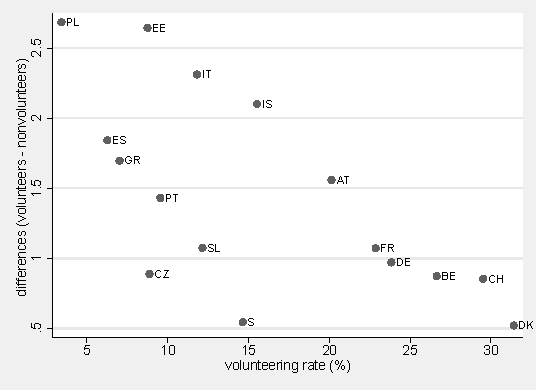
\includegraphics[height=3in]{abs_casp.pdf}
 \centering
% \source{ }
 \label{fig:abs_casp}
\caption{volunteering shares}
\end{figure}


\ref{fig:abs_casp} shows higher heterogeneity of the rates among the low rate countries. The rates in Czech Republic, Portugal and Estonia are very similar but the differences in the condtional means are significantly different. At the same time the rates in Czech Republic and Slovenia are much smaller than in much richer countries such as France, Germany, Luxemburg but the differences in means are at similar levels in all these countries \footnote{Using the relative difference in means does not change conclusion since countries with the highest relative differences are Poland, Estonia, Italy and Isreal and the countries with the smallest differences are: Denmark Sweden,Switzerland, Belgium aand Germany}  \\

\textbf{[AOK: Comment - pls improve it]} A comparison of the volunteering rates with the differences in means present uneasy picture for the interpretation. It seems, as it was concluded in \citet{haski09} and \citet{pagnol10}, that the large rates are associated with smaller impact on wellbeing. It suggests that country specific factors do not play significance role among those countries. Heteregenity seems to be a bigger problem among the low rate countries. This suggests that country specific factors, possibly due to cultural and histotical differences, may play significant role among this coutries. Generally, we expect that "low" influence of voluteering on wellbeing can exist in highly developed countries as well as in less developed ones. However, we do not expect "high" impact from volunteering on QoL in the first group while it may be found in the second. The working explanation is that in highly developed countries formal volunteering is well organized with the efficient help from governmant and many tasks done by volunteers are not of high importance what is not the case among less developed countries. In such countries there more barriers and the demand for truly relevant tasks is much higher. It adds to the fact that volunteers have much stronger feelings of being involved in necessary and highly valued activities. But this is not explains why there is so large heterogenity in the impact among countries where the volunteering is not very popular. This make be related to cultural and historical factors. In the next part of the paper we analyse the relation between the rates of volunteering and its impact on QoL in more detailed way.   

%\textbf{health} \\
%We use similar measure of subjective health to the one used in Haski(2009). This is the self-perceived health variable with the respondents that range from "very bad" to "very good". Subjective health is also higer in more developed countries. In this case people from Southern European countries repored on average highher levels than those from Eastern Europe. The lowes mean values were found for Poland, Estonia, Croatia, Slovenia, Czech Rep. and in Portugal.


\section{Results}

We use the Kendall's tau-b correlation coefficient as a measure of association between the values of the casp index and the binary variable indicationg engagement into volunteering. We apply this measure since the Pearson correlation coefficient may be used only for interval data, while the Kendall's correlation coefficient can be used for either ordinal or interval data. Also, the Kendall's tau is less sensitive to outliers  \citet{khamis08}. The Kendall's tau-b correlation coefficients for the wave 6 of the SHARE data and the Pearson correlations coefficients for the wave 1 from \citet{haski09} are compared below: 


\begin{figure}[H]
\centering
\caption{Volunteering and wellbeing} 
\label{fig:taub}
\begin{minipage}{1\linewidth}
\subfloat[Life satisfaction (\citet{haski09})]{\includegraphics[height=2.7in]{Haski_lifesat.pdf}}\quad
\subfloat[CASP]{\includegraphics[height=2.7in]{Kendall_casp.pdf}}~\\
{\footnotesize Notes: (a) wave 1 (2006-2007), (b) wave 6 (2015) }~\\
{\footnotesize Source: \citet{haski09} [Table 3] and own calculations based on SHARE Wave 6.}
\end{minipage}
\end{figure} 

%
%\begin{figure}[H]
% \includegraphics[height=3in]{Kendall_h.pdf}
% \centering
% \label{fig:tauH}
%\caption{tau subjective health}
%\end{figure}


The Kendall's correlation coefficients range from 15.4\% (Isreal) to 3.3\% (Sweden) what suggests a non-linear association between volunteering and QoL. The significance test allows for some intresting comparisons. For example, the point estimate of association between involvment in volunteering and the level of QoL for Germany (10.9\%) is not statistically different to the association in Slovenia (10.6\%), Spain, Belgium, Portugal, Poland, Switzerland, Croatia and Greece (8.2\%). This is very heterogenouse group  in terms of an economic development and the country rate of volunteering. At the same time the coefficient for Estonia (14.1\%) is statistically different to the coefficients in Slovenia (10.6\%), Poland(9.0\%) and Czech Republic (5.3\%) but it is not different to the values in France, Luxemburg and Austria. Also,the association between volunteering and QoL in Denmark is statistically weaker than in in Spain, Slovenia and Estonia. But it is not different than in Poland or in Czech Republic.  The panel b of Fig 2. clearly shows that such grouping is caused by the strong non-linear shape of the relation between the volunteering rates and    the tau-b coefficient. \\ 

The significance tests confirm the pattern of association between  popularity of volunteering and wellbeing discussed in \citet{haski09}. Results of an analysis based on the more recent data  - we used the data collected in the SHARE survey in 2015 instead of the data from 2006 and 2006 - with more countries, the different measures of volunteering and the association between volunteering and QoL have not chaged the main conclussion from the previouse study. We have shown that the similar impact of volunteering on QoL may co-exist with differnt rates of volunteering. We have found that in countries with the low rates (Czech Republic, Poland) and with the high rates (Denmark, Switzeralnd, Belgium) the association is the same. Also, we have found that the strongest impact of volunteering should be expected in countries with the mid-range rates (Italy, Isreal, Austria) what was not so clearly observed in\citet{haski09}. \\

\citet{haski09} sees two possible explanation of no difference in relation between volunteering and wellbeing according to the rates of volunteering. The first explanation assumes different motives behind volunteering according to the economic developmnent of a country. In countries where the welfare system is strong people volunteer not becouse there are real problems to be solved but becouse there is a such social norm. Lack of necessity is sugested explanation of the weak effect of volunteering.  In countries where the welfare state is weak people involved in volunteering may feel the sense of fullfilment.The second explanation is based on the Social Origins Theory (Salamon and Anheier 1998) and it seems to be similar to the crowding out argument. This argument states that the state through its genorouse social welfare policy satisfies demand for most social needs efficiently constraining supply of volunteering by non-govermental organizations. Both explanations may explain why volunteering can have a limited impact on wellbeing in reach countries. However, they do not tell us why the association may be low in less developed countries. \textbf{[AOK: something is missing here. It would be nice to have some discussion on reasons why the association may be low when the rate is low. Any idea ?]} \\

The differences in socio-economic characteristcs of volunteers and non-volunteers have not been taken into the consideration in the previous discussion. Neither the Pearson's correlation coefficients nor the Kendall's correlation coefficients do not take into account of confounding socio-economic variables that possibly contaminate the relation between volunteering and QoL. Table 3 in the appendix includes descriptives statistics. It shows the significant differences in characteristcs of the two groups. \\

In case of the distributions of age the means are  not statistically different  in Austria, Denmark, Greece, Czech Republic and Portugal . However, the histograms show that the mean is not the good descriptive statistics in this case. In Denmark there is a noticebly larger share of volunteers in the age group of 65-70. In Czech Republic the group of volunteers includes more people in the group age 70-80, while in Portugal there is more people in the age group of 65-75 and in Greece the difference occures for the age group of 55-65. In  all Eastern European countries except Czech Republic the average age of volunteers is below than the age of non-volunteers. In Poland and Estonia there are much larger shares of people in age between 50-55 among volunteers.  In Slovenija the difference is due to smaller share of volunteers older then 70 years. It is interesting since in majority of Western and Southern European  countries (Belgium, France, Germany, Italy, Spain, Switzerland) volunteers are older than non-vilunteers. \\ 

In majority of countries there is no differences in the shares of women among volunteers and non-volunteers. In France and Germany there is larger share of males involved in voluntering while in Grecee, Italy, Spain, Portugal and Sweden we can find more women among volunteers than among non-volunteers. \\

Volunteers are better educated. In all countries average noumber of years in education is higher among volunteers. Also, in each country the share of people with tertiary education is higher among volunteers, while the share of those with primary education is lower. Countries with low volunteering rates are amonh those with the largest difference in a education structure. In Poland the ratio of a share of people with a tertiary  education among volunteers over a share of such people among non-volunteers is 3.49. The respective ratios for Spain, Czech Republic, Estonia are: 2.77, 2.29 and 1.99. The ratios for countries with the high rates of volunteering are smaller. For Denmark it is 1.23, for Belgium it is 1.45, and for Switzerland it is 1.54 \\

Volunteers have better subjective health.  More volunteers declare at least vary good health than non-volunteers. The highest ratio is in Estonia (2.58), Czech Republic (1.61) and Portugal (1.48) and Luxemburg (1.48). The lowest ratio for volunteers over non-volunteers are in Isreal (1.03), Sweden (1.03), Italy (1.09) and Greece (1.10). Distributions of subjective health condtitional on volunteering are somehow puzzeling. There is no clear indication of the relation between a conutry's rate of volunteering and subjective health. For example, the ratio of shares for Poland is between the ratios for Belgium and  Germany and the ratio for Denmark is very similar to that of Spain. Also, the share of people declaring poor health among volunteers is higher in Swededn and Greece than among non-volunteers. The difference in the shares in Portugal is only marginal. On the other hand, in Isreal, Switzerland and Poland the differences in shares are very noticable. \\

Mean group values for income (measured in PPP and with the modified OECD equivalence scale) may be misleading while discussing differences between volunteers and non-volunteers. Using this statistics we conclude that in many countries there are no statistical differences between volunteers and non-volunters. The differences in means are signifcant only for Germany, Isreal and Sweden where volunteers have higher income and in Italy, Spain, Estonia, Switzerland and Luxemburg where they have lower income. However, conditional distributions of equivalized income present much a richer picture. They show that in  all Southern and Eastern European countries there are more people with high income among volunteers than among non-volunteers. This relation holds only for some Western European countries - Austria, Belgium, France, Germany - but even in those cases it is seems to be weaker than among Eastern and Southern European countries. We observe   quite big similarity between the two distributions in Denmark. There is a sign of larger share of people having low income among non-volunteers. Sweden presents a unique case where there is the opposite relation - there are more people with low income among volunteers. The distributions for Germany and Luxemburg reveal another interesting phenomenon. Namely, there is a small group of very rich people among non-volunteers that does not exist among volunteers. \footnote{Volunteering dash line} \textbf{[AOK: Add to your list of possible follow-up papers : Donating money v donating time] } \\

\textbf{[Missing summary of what above. It should show how large are differences among countries Also, it may stress differences between "rich" and "poor" countries and between "former socialistic" and "southern europe" on one side, and "western europe" on the other.]}

 
% Casp v volunteering


%Volunteers give on average better answer about subjective health. Comparing conditional mean scores reveals different pattern to the one discussed for casp. There is weaker relation between popularity of volunteering in a country and its impact on subjective health. 

%\begin{figure}[H]
%\centering
%\caption{Unconditional means} 
%\label{fig:vol_casp}
%\begin{minipage}{1\linewidth}
%\subfloat[CASP]{\includegraphics[height=2.7in]{rel_casp.pdf}}\quad
%\subfloat[CASP]{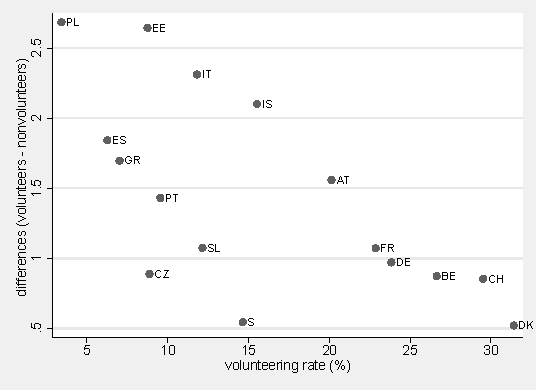
\includegraphics[height=2.7in]{abs_casp.pdf}} \quad
%\subfloat[Health]{\includegraphics[height=2.7in]{rel_health.pdf}}\quad
%\subfloat[Health]{\includegraphics[height=2.7in]{abs_health.pdf}} ~\\
%{\footnotesize Notes: }~\\
%{\footnotesize Source: Own calculations based on SHARE Wave 6.}
%\end{minipage}
%\end{figure} 

\subsection*{Volunteering and casp (regression analysis)}

We have shown that volunteers and non-volunteers differ in their  socio-economic characteristics.. Also, we have shown that  the ways how they differ are different in countries. In the first part of the paper we have arqued that the impact of volunteering on QoL is differes among countries. Now, we want to combine these two findings and to ask wheter the differences in the characteristics influence the variation of relation between volunteering and QoL in the countries' volunteering rate. We analyze that relation with two different asumptions. Firstly, we assume that the it is possible to identify the common for all countries relation between volunteering and QoL. In this approach the country effect depends on explantory variables and any deviation from its conditional expected value is treated as a random event. Also, it means that the deviations from the grand mean are not related to country characteristics incuded in a model. This assumption leads to the random effect specification.  The second approach assumes that the universal relation for each country can not be identified and that for each country we have the separate relation. Here, the country effect encompasses the differences in history, cultural factors and institutions that are seen as the unique characteristic of a country. This is consistent with findings that "contextual factors, such as a country’s historical background or institutions, determine levels of volunteering to a large extent" (\citet{plagnol10}). This assumption leads to the fixd effect specification in which the estimates for one country give us no information on the effect for other ones. The fixed effect approach does not allow for predicing changes in relation between volunteering and QoL in a given country using the predictions for other countries. \\

The first approach can specifies as a multilevel linear regression model. Below we consider a model with a varying intercept for countries and varying coefficient for impact of volunteering on QoL. Random intercept for each country allows for different values of QoL within a country by gender, age and other control variables. In the model we make the volunteering parameter to depend on the rate of volunteering :

 \begin{eqnarray}
  \label{eq:casp_mlm}
	casp_{i,c}\sim N(\beta_{0}+ u_{c} +  \beta_{1,c} * vol_{i,c}+\gamma*Z_{i,c},\sigma^{2}_{y}) \\	
	\beta_{1,c} \sim N(\gamma_{r}*ln(r_{c}),\sigma^{2}_{r})
 \end{eqnarray}
 
where $r_{c}$ is a country volunteering rate calculted from the wave 6 of the SHARE survey. \\ 

The second approach is equivalent to the estimation of the separate models for each country : 
 
  \begin{eqnarray}
	casp_{i,c}= \beta_{0c}+ \beta_{1c}*v_{i,c} + \gamma_{c}*Z_{i,c} + \epsilon_{i,c}
 \end{eqnarray}

where $v_{i,c}$ is a binary variable equal to 1 if a person i from a country c is involved in  volunteering  and a matrix $Z_{i,c}$ includes the following controls : age, gender, education measured in years of formal educatin, a country average gdp per capita expressed in purchasing power parity in years X-Y and a equivalized houseshold level income also in ppp units.  In the model $\beta_{0c}$ controls for country-specific factors   and $\beta_{1c}$ describes impact of volunteering on QoL. For each country we get the separate coefficient while controlling for the general country effect $\beta_{0c}$ and a set of confounders. No restrictions are assumed on the variance of the error terms for each country. \\

Below we compare results from both models \\ 
%%%%%%%%%%%%%%%%%%  LINEAR REGRESSION (Separate models) %%%%%%%%%%%%%%%%%%%%%%%%%

\begin{spacing}{.9}
\begin{table}[H]
\centering 
\caption{CASP vs. volunteering (OLS)- part 1}  
\begin{scriptsize} 
	 {
\def\sym#1{\ifmmode^{#1}\else\(^{#1}\)\fi}
\begin{tabular}{l*{9}{c}}
\hline\hline
                    &\multicolumn{1}{c}{(1)}&\multicolumn{1}{c}{(2)}&\multicolumn{1}{c}{(3)}&\multicolumn{1}{c}{(4)}&\multicolumn{1}{c}{(5)}&\multicolumn{1}{c}{(6)}&\multicolumn{1}{c}{(7)}&\multicolumn{1}{c}{(8)}&\multicolumn{1}{c}{(9)}\\
                    &\multicolumn{1}{c}{casp}&\multicolumn{1}{c}{casp}&\multicolumn{1}{c}{casp}&\multicolumn{1}{c}{casp}&\multicolumn{1}{c}{casp}&\multicolumn{1}{c}{casp}&\multicolumn{1}{c}{casp}&\multicolumn{1}{c}{casp}&\multicolumn{1}{c}{casp}\\
\hline
vol                 &        1.04***&        0.51** &        0.28*  &        0.54** &        0.62***&        1.70***&        1.65***&        1.93***&        1.30***\\
ageint              &       -0.02+  &        0.03***&        0.01   &        0.01   &        0.03** &       -0.05***&        0.06** &       -0.01   &       -0.06***\\
Male or female      &       -0.24   &       -0.17   &        0.23+  &       -0.43*  &       -0.01   &       -0.63***&       -0.04   &       -0.54** &       -0.20   \\
yedu\_av             &       -0.05** &        0.04+  &       -0.03   &        0.12***&        0.07***&        0.12***&        0.24***&        0.12***&        0.07***\\
1b.sphus            &        0.00   &        0.00   &        0.00   &        0.00   &        0.00   &        0.00   &        0.00   &        0.00   &        0.00   \\
2.sphus             &       -0.91** &       -0.86** &       -1.38***&       -0.64+  &       -0.89*  &       -1.29***&       -1.17*  &       -1.93***&       -0.38   \\
3.sphus             &       -2.46***&       -2.53***&       -2.22***&       -2.12***&       -2.25***&       -2.63***&       -0.84   &       -2.68***&       -2.18***\\
4.sphus             &       -4.99***&       -5.13***&       -3.95***&       -4.42***&       -4.53***&       -4.76***&       -1.98** &       -4.66***&       -4.40***\\
5.sphus             &       -6.10***&       -8.32***&       -6.25***&       -6.25***&       -7.01***&       -6.32***&       -4.80***&       -6.04***&       -7.27***\\
constant            &       45.32***&       40.14***&       43.12***&       40.55***&       40.12***&       38.89***&       30.43***&       39.56***&       43.52***\\
\hline
N                   &        2534   &        4038   &        3029   &        2648   &        3460   &        3411   &        1188   &        3616   &        3696   \\
\hline\hline
\end{tabular}
}

      \label{SepMod} 
\end{scriptsize}
\end{table}
\end{spacing}
%%% END: TABLE

\begin{spacing}{.9}
\begin{table}[H]
\centering 
\caption{CASP vs. volunteering (OLS) - part 2}  
\begin{scriptsize} 
	 {
\def\sym#1{\ifmmode^{#1}\else\(^{#1}\)\fi}
\begin{tabular}{l*{8}{c}}
\hline\hline

                                &         S   &          CH   &          CZ   &           PL   &          LU  &          PT  &          SL  &           EE    \\
\hline
vol                 &        0.64** &        0.46*  &        0.48+  &        1.62*  &        0.40   &        1.18*  &        0.70** &        1.41***\\
age                 &       -0.04***&        0.00   &       -0.01   &        0.01   &        0.05***&       -0.00   &       -0.03** &       -0.03** \\
female              &        0.28+  &       -0.17   &       -0.07   &       -0.28   &        0.20   &        0.01   &       -0.00   &        0.76***\\
edu                 &       -0.08***&       -0.01   &       -0.02   &        0.23***&        0.06*  &        0.04   &        0.11***&        0.06*  \\
1b.sphus            &        0.00   &        0.00   &        0.00   &        0.00   &        0.00   &        0.00   &        0.00   &        0.00   \\
2.sphus             &       -0.95***&       -0.95** &       -1.24** &       -1.17   &       -1.35** &       -1.82*  &       -0.93*  &       -1.39*  \\
3.sphus             &       -2.51***&       -2.92***&       -2.87***&       -3.19** &       -2.74***&       -2.56***&       -2.82***&       -2.50***\\
4.sphus             &       -3.96***&       -4.52***&       -4.19***&       -5.03***&       -4.63***&       -4.12***&       -4.23***&       -4.57***\\
5.sphus             &       -6.06***&       -5.33***&       -6.73***&       -7.16***&       -7.51***&       -6.87***&       -6.44***&       -7.40***\\
income              &        0.02***&        0.00   &        0.05*  &        0.00   &       -0.00+  &        0.01*  &        0.01   &        0.15***\\
constant            &       44.90***&       43.57***&       40.12***&       39.23***&       39.94***&       38.49***&       43.35***&       40.44***\\
\hline
N                   &        3096   &        2220   &        3541   &        1103   &        1139   &         907   &        3031   &        3527   \\
\hline\hline
\end{tabular}
}

      \label{SepMod1} 
\end{scriptsize}
\end{table}
\end{spacing}
%%% END: TABLE


%%%%%%%%%%%%%%%%%%  MLM %%%%%%%%%%%%%%%%%%%%%%%%%

%%% TABLE
\begin{spacing}{.9}
\begin{table}[H]
\centering 
\caption{Wellbeing v. volunteering (Multilevel Linear Model)}  
\begin{scriptsize} 
	 {
\def\sym#1{\ifmmode^{#1}\else\(^{#1}\)\fi}
\begin{tabular}{l*{1}{c}}
\hline\hline
            &\multicolumn{1}{c}{casp}\\
\hline
volunteering&        0.90***\\
age: 60-70  &        0.42***\\
age: 71+    &       -0.08   \\
female      &       -0.08+  \\
edu         &        0.06***\\
health:excellent&        6.82***\\
health:very good&        5.74***\\
health:good &        4.35***\\
health:fair &        2.37***\\
income      &        0.00***\\
gdp         &        0.25***\\
gdp sq      &       -0.00** \\
BE          &       -1.74***\\
DK          &       -0.12   \\
FR          &       -1.54***\\
DE          &       -0.81** \\
S           &       -1.24***\\
CH          &        1.70   \\
LU          &       21.96*  \\
GR          &       -6.87***\\
IS          &       -4.48***\\
PT          &       -3.02***\\
IT          &       -3.83***\\
ES          &       -2.47***\\
CZ          &       -3.10***\\
PL          &        1.38** \\
constant    &       22.27***\\
sd(vol)     &        0.23***\\
sd(Residual)&        4.51***\\
\hline
N           &       45764   \\
\hline\hline
\end{tabular}
}

      \label{regB} 
\end{scriptsize}
\end{table}
\end{spacing}
%%%% END: TABLE

%%%%%%%%%%%%%%%%%%  MLM %%%%%%%%%%%%%%%%%%%%%%%%%


Volunteering has a positive impact on QoL regardles the approach has been chosen. The multilevel model estimated is 0.91 and is it statistically significant at the level less than 1\%. The fixed effect approach estimates range from 0.28 for Denmark to 1.84 for Italy. All coefficients are significant except the one for Luxemburg. The high point estimates are for the low rate countries such as: Greece, Italy, Spian, Isreal, Poland, Estonia. The low estimates are for: Denmark, Belgium, Germany, Switzerland and Czech Republic. \\

Estimates on the control socio-economics variables have expected signs. Better subjective health and higher income increase QoL. Age is positively related to QoL in rich countries - Belgium, Danmark, Germany, Isreal, Luxemburg - and negatively in Austria, Greece, Spain, Sweden, Czech Rep.,  Slovenia, Estonia. In Poland, Switzerland, Portugal, France, Italy the age variable has appeared to be insignificant. In the random effect approach the age effect  showed up with the minus sign. The female effect turned out to have different directions among the analysed countries, also.  It has shown higher impact for women in two Scandinavic countries - Denmark and Sweden - and in Estonia. Average effect from the random effect approach suggests lower impact for women. In majority of countries education showed positive effect on QoL. Only in Austria, Denmark, Sweden we get statistically significant negative values. Income has either positive effect or it has no effect on QoL. \\    

The fixed effect approach allows us to decompose the within country difference in means of QoL  into the volunteering effect and the effect due to differences in characteristics (the endowment effect): \footnote{It is possible since $\bar{casp_{c}} = \bar{\hat{casp_c}}$} 

 \begin{eqnarray}
 \label{eq:casp_ols}
E[casp_{c}|v_{i,c}=1] - E[casp_{c}|v_{i,c}=0]= \beta_{1c}+ \gamma_{c}*[\bar{Z}_{c}(1)-\bar{Z}_{c}(0)]
 \end{eqnarray}

with $\bar{\hat{casp_{c}}}(1)$ being a predicted average QoL for a volunteer and $\bar{\hat{casp_{c}}}(0)$ being a predicted average QoL for a non-volunteer.  The first term measures the volunteering effect for country c, the second term absorbs the effect of the difference in the values of covariates among volunteers and non volunteers (the endowment effect) with $\bar{Z}_{c}(1)$ being average endowment among volunteers and $\bar{Z}_{c}(0)$ among non-volunteers. \\

The mean difference in QoL in the random effect approach can be decomposed as: 

 \begin{eqnarray}
 \label{eq:decomp_mlm}
E[casp_{c}|v_{i,c}=1]-E[casp_{c}|v_{i,c}=0]= [\beta_{1}+u_{r}(c)]+ \gamma*(\bar{Z}_{c}(1)-\bar{Z}_{c}(0))+ [\bar{\epsilon}_{i,c}(1)-\bar{\epsilon}_{i,c}(0)]
 \end{eqnarray}

\begin{figure}[H]
\centering
\caption{Volunteering and wellbeing (OLS)} 
\label{fig:casp_ols}
\begin{minipage}{1\linewidth}
\subfloat[Fixed effect model]{\includegraphics[height=2.7in]{ols_fitcry.pdf}}\quad
\subfloat[Random effect model]{\includegraphics[height=2.7in]{mlmQ_fit0.pdf}}~\\ 
{\footnotesize Notes: }~\\
{\footnotesize Source: Own calculations based on SHARE Wave 6.}
\end{minipage}
\end{figure} 

The results from both models are consistent with the previouse finding on a weak relation between volunteering and QoL in highly developed countries. This conclusion is robust to the used approach in modelling. However, the models disagree in the  predictions of importance of volunteering in the low rate countries. Controlling for confounders in the fixed effect approach shows rather decreasing relation between popularity of volunteering at a country level and its impact on QoL.  It shows higher effect in Italy, Greece, Isreal and Poland than in the countries with the higher rates such as Denmark, Switzerland, Luxemburg, Sweden. This negative relation is consistent with the two explanations given in the \citet{haski09}. On the other hand, the random effect approach gives us a solution resembling a non-linear relation with the highest impact in Italy and Isreal. In countries with low rates and in these where they are high the impacta are weaker. This makes the results from the random effect model a bit like those obtained with the Kendall's correlations. \\

Controlling for age, gender, education, economic development of a country and household's income generally decreases an impact of volunteering in QoL. The fixed effect approach suggests especially significant effect of a selection into volunteering in Poland and Estonia. Selection is also important in highly developed countries like Luxemburg and France. The selection effect seems to have smaller role in Italy, Greece, Spain, Portugal and Isreal. In Sweden the selection plays a minor role what has been expected after comparing the socio-economic characteristics of volunteers and non-volunteers. It is intresting that in two formerly socialistic countries - Poland and Estonia - selection into volunteering is more important than in Southern Europe. It suggests that nowdays volunteering of elderly in CEE coutries adds reltively less to average QoL  than in Southern Europe. It may be becouse volunteers in CEEs are more often selected from those who had high level of QoL even without the volunteering. This may be realted to weak infrastruture for volunteering in these countries what, as was pointed in \citet{plagnol10}, causes that only highly motivated individuals engage in voluntary activities. \\ 


% It seems that in countries where the rates of volunteering are low - Poland, Spain, Greece, Estonia - the large difference in the levels of QoL are in large part due to the differences in characteristics. This means that volunteers had had higher QoL than non-volunteers even if they would not be involved in volunteering. The role of unobserved characteristics is noticebly important in Poland. In Italy and Isreal the volunteering effect explains larger part of the differences in QoL than in other countries. The volunteering effect is weak among countries with the large rates of volunteering except Denmark. The Danish effect is larger than the effects in Switzeralnd, Belgium, Luxemburg, Germany, France and Austria. Its absolute level is simialar to the levels in four countries with the smallest rates. \\
   
 
\section{Discussion}

We applied three empirical methods to discuss an association of volunteering with QoL. Firstly, we calculated the Kendall tau-b correlation coefficients and compared  our results with those discussed in \citet{haski09}. Then, we applied a multivariate linear approach to QoL with a set of controls for socio-economic characteristics as exogenouse variables. We estimated the model with two different specifications -  as the fixed effect model and as the random effect one.\\

We were interested in the two issues in this study: a) whether the relation between volunteering rates for elderly and QoL differ according to countires and b) how that relation changes in the volunteering rates. We found the support for our first hypothesis regardless of the method used. The results of the Kendall tau-b correlation analysis as well as the esimates of a multivariate liner regression models showed higher QoL among volunteers. They showed different associatin between volunteering and QoL according to countries, too. This variation between countries was observed even after controling for socio-demographic characteristics such as age, education, gender and income. Our results are in line with the previouse studies (\citet{haski09}, \citet{plagnol10}). The multivariate approach reveals that part of an unconditional correlation between volunteering and QoL may be explained by the selection of people into the voluntareeing sector. Not taking into account difefrences in characteristics between volunteers and non-volunteers leads to the overestimation of the impact of voluntering on QoL since volunteers are recruited from people whose characteristics are positivly correlated with QoL. Our study showed that the significance of selection effect differs according to countries. Despite that, the volunteering effect on QoL is still quite strongly diverse according to countries even after controlling for possible effect due to selection. \\

We did not find the clear answer for the second question. Both regression approaches suggested the weaker volunteering effect in countries with high rates. This conlusion seems to be robust in all applied methods. Conclussions differ in regard of countries with the low volunteering rates.The fixed effect approach, that assumes significant role for country specific cultural and historical factors, showed stronger effect in those countries than in the first group.This is consistent with the statment in \citet{plagnol10} that stress the role of selection into the volunteering sector - " ... volunteers in countries with a low frequency of volunteering displayed higher values on several of the wellbeing measures than those in other countries. (...) in countries where volunteering is generally less common, those who do participate in formal or informal volunteering have the highest levels of well-being. It may be that in these countries, only those who are most likely to benefit from volunteering actually volunteer". Unfortunately the fixed effect approah does not allow us to predict what would be the effect of increasing popularity of volunteering in these countries on the basis of the results for other countries. But some speculative conclussion may be rised from the random effect approach that assumes the common model for all countries. The result of that approach suggests the strongest association between voluntering and QoL among countries with the mid-range volunteering rates. Hence, we allow that increasing the popularity of volunteering in countries where the current rates are low may decrease in averege impact of it on QoL but we do not expect this to be significance in size.  \\    

We belive that one issue in regard of the relation between volunteering and QoL rised in the study needs the speciall attantion. This study is built up on the previous research discussed in \citet{haski09}. Our study extends it by considering Central and Eastern European countries. The volunteering rates are low in all these countries. This made the sample of countries more diverse. We showed that the shares of volunteers in the age group of 50-65 in Poland, Estonia and Slovenia are rather high. The shares of older elderly - in age 70+ - in those countries are low. All of the above findings - low volunteering rates and age structure - may be related to age cohort effects. Particpants of the SHARE survey analysed in the study had their working career years during the socialistic regime. This might have two negative consequences on their wilingness to paricipate in volunteering. First, volunteering can badly associate them. Secondly, they are in bad health due to poor working conditions in the past (Wahrendorf, 2016). These factors make the population of elderly in CCE in the studied sample significantly different to their peers (równieśnicy) in other european countries. But we may assume that they are much different to future elderly in CEE whose will be much like their peers from Western Europe. All of these suggests that we may be in favor of the fixed effect approach for the current analysis that's goal is to describe differences among countries. At the same time we may prefer  the random effect model when we are looking for predictioni how volunteering will influence QoL in countries where the current rates are low. \\

It is unfortunate that the volunteering is not very popular among elderly in less developed European countries. However if our understanding of the selection into volunteering is correct we should expect increase in the rates even without any special public policy.  




\begin{thebibliography}{87}
\newcommand{\enquote}[1]{``#1''}
\expandafter\ifx\csname natexlab\endcsname\relax\def\natexlab#1{#1}\fi

\bibitem[\protect\citeauthoryear{Anderson, Damianakis, Kr{\"o}ger, Wagner, Dawson, Binns, Bernstein, Caspi, and Cook}{Anderson et~al.}{2014}]{anderson14}
\textsc{Anderson, N.~D., T.~Damianakis, E.~Kr{\"o}ger, L.~M. Wagner, D.~R.Dawson, M.~A. Binns, S.~Bernstein, E.~Caspi, and S.~L. Cook} (2014):  \enquote{The benefits associated with volunteering among seniors: a critical  review and recommendations for future research.} \emph{Psychological bulletin}, 140, 1505.

\bibitem[\protect\citeauthoryear{Bergmann, Kneip, De Luca, and Scherpenzeel}{Bergmann et~al.}{2017}]{bergmann17}
\textsc{Bergmann, M., T.~Kneip, G.~De Luca, A.~Scherpenzeel} (2017):  \enquote{Survey participation in the Survey of Health, Ageing and Retirement in Europe (SHARE), Wave 1-6.} \emph{Working Paper Series}, 31-2017.


\bibitem[\protect\citeauthoryear{Borgonovi}{Borgonovi}{2008}]{borgonovi08}
\textsc{Borgonovi, F.} (2008): \enquote{Doing well by doing good. The relationship between formal volunteering and self$-$reported health and happiness,} \emph{Social Science and Medicine}, 66,  2321 -- 2334.

\bibitem[\protect\citeauthoryear{Borrat-Besson, Ryser and Gonçalves}{Borrat-Besson et~al.}{2015}]{borrat15}
\textsc{Borrat-Besson, C.,V-A.~Ryser, and J.~Gonçalves} (2015):  \enquote{What impact does it really have?} \emph{An evaluation of the CASP-12 scale used in the Survey of Health, Ageing and Retirement in Europe (SHARE) to measure Quality of Life among people aged 50+}, \emph{FORS Working Papers}, 2015-4


\bibitem[\protect\citeauthoryear{Casiday, Kinsman, Fisher and Bambra}{Casiday et~al.}{2008}]{casiday08} 
\textsc{Casiday, R., E.~Kinsman, C.~Fisher and C.~Bambra} (2008):  \enquote{What impact does it really have?} \emph{Report to Volunteering England}, London: Volunteering England.

\bibitem[\protect\citeauthoryear{Detollenaere, Willems, Baert}{Detollenaere et~al.}{2017}]{detollenaere17}
\textsc{Detollenaere, J. and S.~Willems and S.~Baert} (2017): \enquote{Volunteering, income and health,} \emph{PLoS ONE}, 12(3):e0173139,  doi:10.1371/journal.pone.0173139.

\bibitem[\protect\citeauthoryear{Ehlers, Naegele, Reichert}{Ehers et~al.}{2011}]{ehlers11}
\textsc{Ehlers, A. and G.~Naegele and M.~Reichert} (2011): \enquote{Volunteering by older people in the EU,} \emph{European Foundation for the Improvement of Living and Working Conditions} 

Ehlers, Anja; Naegele, Gerhard; Reichert, Monika

\bibitem[\protect\citeauthoryear{Haski-Leventhal}{Haski-Leventhal}{2009}]{haski09}
\textsc{Haski-Leventhal, D.} (2009): \enquote{Elderly volunteering and
  well-being: A cross-European comparison based on SHARE data,} \emph{Voluntas:
  International Journal of Voluntary and Nonprofit Organizations}, 20, 388--404.
  
  % Potwierdzeni CASP in SHARE
%@article{doi:10.1080/13607863.2017.1292208,
%author = {Gema Pérez-Rojo and Noemy Martín and Cristina Noriega and Javier López},
%title = {Psychometric properties of the CASP-12 in a Spanish older community dwelling sample},
%journal = {Aging \& Mental Health},
%volume = {0},
%number = {0},
%pages = {1-9},
%year  = {2017},
%abstract = {Objective: Current studies have shown that older people's quality of life (QoL) is more associated to individual's sense of happiness and subjective life satisfaction than to objective problems. CASP scale conceptualizes QoL based on a psycho-sociological perspective. Originally, CASP consisted of 19 items (four factors: Control, Autonomy, Self-realization and Pleasure). Later, it was proposed a shorter version (12 items and three factors). The aim of this study was to assess the structure of the CASP-12 SHARE version using confirmatory factor analysis.  
  
\bibitem[\protect\citeauthoryear{Hank and Erlinghagen}{Hank and   Erlinghagen}{2009}]{hank09}
\textsc{Hank, K. and M.~Erlinghagen} (2009): \enquote{Dynamics of volunteering in older Europeans,} \emph{The Gerontologist}, 50, 170--178.  

\bibitem[\protect\citeauthoryear{Hyde}{Hyde}{2003}]{hyde03}
\textsc{Hyde, M.} (2003): \enquote{A measure of quality of life in early old age: The theory, development and properties of a needs satisfaction model (CASP-19),} \emph{Aging and mental health}, 7(3), 186--194. 


\bibitem[\protect\citeauthoryear{Jenkinson, Dickens, Jones, Thompson-Coon, Taylor, Rogers, Bambra, Lang, and Richards}{Jenkinson et~al.}{2013}]{jenkinson2013volunteering}
\textsc{Jenkinson, C.~E., A.~P. Dickens, K.~Jones, J.~Thompson-Coon, R.~S.Taylor, M.~Rogers, C.~L. Bambra, I.~Lang, and S.~H. Richards} (2013):
  \enquote{Is volunteering a public health intervention? A systematic review and meta-analysis of the health and survival of volunteers,} \emph{BMC public health}, 13, 773.

% Khamis H. Measures of Association: How to Choose? Journal of Diagnostic Medical Sonography. 2008;24:155-162.}

\bibitem[\protect\citeauthoryear{Li and Ferraro}{Li and Ferraro}{2006}]{li06}
\textsc{Li, Y. and KF.~Ferraro} (2006): \enquote{Volunteering in middle and later life: is health a benefit, barrier or both ?} \emph{Social Forces}, 85, 497--519. 


\bibitem[\protect\citeauthoryear{Meier and Stutzer}{Meier and
  Stutzer}{2008{\natexlab{b}}}]{meier08}
---\hspace{-.1pt}---\hspace{-.1pt}--- (2008{\natexlab{b}}): \enquote{Is volunteering rewarding in itself?} \emph{Economica}, 75, 39--59.

\bibitem[\protect\citeauthoryear{Morrow-Howell, Hinterlong, Rozario and Tang}{Morrow-Howell et~al.}{2003}]{morrow2003}
\textsc{Morrow-Howell, N., J.~Hinterlong, P.~A.Rozario, F.~Tang} (2003):
  \enquote{Effects of Volunteering on the Well-Being of Older Adults,} \emph{The Journals of Gerontology: Series B},58, S137--S145

\bibitem[\protect\citeauthoryear{National Research Council (US) Panel on a Research Agenda and New Data for an Aging World}{National Research Council (US)}{2001}]{nrc2001}
\textsc{National Research Council (US) Panel on a Research Agenda and New Data for an Aging World)} (2001):
  \enquote{Preparing for an Aging World: The Case for Cross-National Research. ,} \emph{Washington (DC): National Academies Press (US)},2001, Available from: https://www.ncbi.nlm.nih.gov/books/NBK98384/


\bibitem[\protect\citeauthoryear{Oecd}{Oecd}{2015}]{Oecd15}
\textsc{Oecd} (2015): \enquote{How's Life  2015 - Measuring Well-being} \emph{OECD 2015}.

\bibitem[\protect\citeauthoryear{Oecd}{Oecd}{2016}]{Oecd16}
\textsc{Oecd} (2016): \enquote{Society at Glance} \emph{OECD 2016}.

 \bibitem[\protect\citeauthoryear{Plagnol and Huppert}{Plagnol and Huppert}{2010}]{plagnol10}
\textsc{Plagnol, A. C. and ~F-A.Huppert } (2010): \enquote{Happy to help? Exploring the factors associated with variations in rates of volunteering across Europe,} \emph{Social Indicators Research}, 97(2), 157--176.
  
 \bibitem[\protect\citeauthoryear{Prouteau and Wolff}{Prouteau and Wolff}{2006}]{prouteau06}
\textsc{Prouteau, L. and ~F-C.Wolff } (2006): \enquote{Does volunteer work pay off in the labor market?,} \emph{Journal of Socio-Economics}, 35, 992--1013.

\bibitem[\protect\citeauthoryear{Salamon, Haddock, and Sokolowski}{Salamon et~al.}{2017}]{salomon2017} \textsc{Salamon, L.~M., M.~A. Haddock and W.~S. Sokolowski}(2017):
 \enquote{Closing the Gap? New Perspectives on Volunteering North and South,} \emph{J. Butcher, C.J. Einolf (eds.), Perspectives on Volunteering, Nonprofit and Civil Society Studies, $DOI 10.1007/978-3-319-39899-0_2$}, chapter 2, 29--51.
  
\bibitem[\protect\citeauthoryear{Thoits and Hewitt}{Thoits and Hewitt}{2001}]{thoits03}
\textsc{Thoits, P.A. and ~L.N.Hewitt } (2001): \enquote{Volunteer Work and Well-Being,} \emph{Volunteer Work and Well-Being},42, 115--131.


\bibitem[\protect\citeauthoryear{Whillans, Seider, Chen, Dwyer, Novick, Gramign, Mitchell, Savalei, Dickerson and Dunn}{Whillans et~al.}{2016}]{whillans2016}
\textsc{Whillans, A.~V., S.~C. Seider, L.~Chen, R.~J. Dwyer, S.~Novick, K.~J.Gramign, B.~A. Mitchell, V.~Savalei, S.~S.Dickerson and E.~W. Dunn}(2016):
  \enquote{Does volunteering improve well-being?,} \emph{omprehensive Results in Social Psychology}, 1, 35--50.

  
\bibitem[\protect\citeauthoryear{Wilson}{Wilson}{2012}]{wilson12}
\textsc{Wilson, J.} (2012): \enquote{Volunteerism research: A
  review essay,} \emph{Nonprofit and Voluntary Sector Quarterly}, 41, 176--212.

\bibitem[\protect\citeauthoryear{Ziemek}{Ziemek}{2006}]{ziemek06}
\textsc{Ziemek, S.} (2006): \enquote{Economic analysis of volunteers` motivations. A cross$-$country study,} \emph{Journal of Socio$-$Economics}, 35(3), 532--555.


\bibitem[\protect\citeauthoryear{Van Willigen}{Van Willigen}{2000}]{VanWilligen00}
\textsc{Van Willigen, M.} (2000): \enquote{Differential benefits of volunteering across the life course,} \emph{Journal of Gerontology Series B}, 55, 5308--5318.


\end{thebibliography}


\begin{spacing}{.9}

\section{Appendix: additional descriptive statistics}


%%%%%%%%%%%%%%%%%%%%%%%%%%%%%%%%%%%%%%%%%%%%%%%%%%%%%%%%%%%%%%%%
% Rozkład CASP
\begin{figure}[H]
 \includegraphics[height=3in]{hist_casp.pdf}
 \centering
 \label{fig:hist_casp}
\caption{Distribution of CASP by countries}
\end{figure}

%%% TABLE: Kendall tau-b
\begin{spacing}{.9}
	 % Table generated by Excel2LaTeX from sheet 'casp'
\begin{table}[htbp]
  \centering
  \caption{Significance test - Kendall tau correlations}
    \begin{tabular}{lrccccccccccccccccc}
          &       & IT    & AT    & EE    & FR    & LU    & DE    & SL    & SE    & BE    & PT    & PL    & CH    & CR    & GR    & DK    & CZ    & S \\
    IS    & 15.4 & 64.1 & 58.4 & 54.2 & 19.0 & 15.8 & \textbf{5.0} & \textbf{3.6} & \textbf{2.1} & \textbf{1.8} & \textbf{5.3} & \textbf{1.5} & \textbf{0.6} & \textbf{0.4} & \textbf{0.2} & \textbf{0.0} & \textbf{0.0} & \textbf{0.0} \\
    IT    & 14.4 & X     & 87.9 & 83.8 & 23.7 & 20.7 & \textbf{3.6} & \textbf{2.2} & \textbf{0.9} & \textbf{0.6} & \textbf{5.7} & \textbf{1.0} & \textbf{0.3} & \textbf{0.1} & \textbf{0.0} & \textbf{0.0} & \textbf{0.0} & \textbf{0.0} \\
    AT    & 14.1 &       & X     & 98.0 & 36.2 & 28.2 & \textbf{8.9} & \textbf{6.1} & \textbf{3.4} & \textbf{2.6} & \textbf{9.5} & \textbf{2.5} & \textbf{0.9} & \textbf{0.5} & \textbf{0.1} & \textbf{0.0} & \textbf{0.0} & \textbf{0.0} \\
    EE    & 14.1 &       &       & X     & 31.9 & 25.9 & \textbf{5.7} & \textbf{3.7} & \textbf{1.6} & \textbf{1.2} & \textbf{7.8} & \textbf{1.6} & \textbf{0.4} & \textbf{0.2} & \textbf{0.0} & \textbf{0.0} & \textbf{0.0} & \textbf{0.0} \\
    FR    & 12.3 &       &       &       & X     & 69.8 & 43.4 & 33.6 & 24.0 & 20.3 & 33.2 & 13.6 & \textbf{6.7} & \textbf{4.4} & \textbf{2.2} & \textbf{0.2} & \textbf{0.0} & \textbf{0.0} \\
    LU    & 11.4 &       &       &       &       & X     & 85.5 & 74.9 & 65.6 & 60.6 & 63.6 & 39.6 & 28.6 & 22.9 & 19.7 & \textbf{4.9} & \textbf{1.3} & \textbf{0.1} \\
    DE    & 10.9 &       &       &       &       &       & X     & 84.7 & 71.1 & 63.6 & 69.2 & 38.0 & 23.8 & 17.3 & 11.7 & \textbf{1.5} & \textbf{0.1} & \textbf{0.0} \\
    SL    & 10.6 &       &       &       &       &       &       & X     & 87.0 & 79.1 & 80.1 & 47.3 & 31.5 & 23.6 & 17.5 & \textbf{2.5} & \textbf{0.3} & \textbf{0.0} \\
    SE    & 10.3 &       &       &       &       &       &       &       & X     & 91.4 & 88.7 & 53.8 & 36.2 & 27.2 & 20.1 & \textbf{2.7} & \textbf{0.2} & \textbf{0.0} \\
    BE    & 10.1 &       &       &       &       &       &       &       &       & X     & 94.5 & 59.3 & 41.0 & 31.2 & 24.1 & \textbf{3.5} & \textbf{0.3} & \textbf{0.0} \\
    PT    & 10.0 &       &       &       &       &       &       &       &       &       & X     & 72.2 & 57.8 & 48.9 & 45.9 & 14.5 & \textbf{4.8} & \textbf{0.6} \\
    PL    & 9.0 &       &       &       &       &       &       &       &       &       &       & X     & 84.3 & 73.2 & 71.4 & 24.6 & \textbf{8.5} & \textbf{1.1} \\
    CH    & 8.6 &       &       &       &       &       &       &       &       &       &       &       & X     & 87.9 & 87.5 & 30.9 & 10.5 & \textbf{1.2} \\
    CR    & 8.2 &       &       &       &       &       &       &       &       &       &       &       &       & X     & 98.9 & 38.7 & 14.3 & \textbf{1.8} \\
    GR    & 8.2 &       &       &       &       &       &       &       &       &       &       &       &       &       & X     & 31.6 & \textbf{8.7} & \textbf{0.6} \\
    DK    & 6.4 &       &       &       &       &       &       &       &       &       &       &       &       &       &       & X     & 54.6 & 10.9 \\
    CZ    & 5.3 &       &       &       &       &       &       &       &       &       &       &       &       &       &       &       & X     & 28.1 \\
    S     & 3.3 &       &       &       &       &       &       &       &       &       &       &       &       &       &       &       &       & X \\
    \end{tabular}%
  \label{tab:addlabel}%
\end{table}%

      \label{KendallCasp} 
\end{spacing}
%%%% END: TABLE



%%%%%%%%%%%%%%%%%%%  DESCRIPTIVES %%%%%%%%%%%%%%%%%%%%%%%%%

 
%%% TABLE
\begin{spacing}{.9}
\centering 
\begin{tiny} 
	 % matrix: Desc0 file: C:\projekty\NCN_AdamOK\wyniki\Papers\Paper2_Haski\tex\descTtest0.tex   6 Apr 2018 12:02:37
\begin{table}[htbp]
\caption{\label{clabel} Descriptive statistics}\centering\medskip
\begin{tabular}{lccccccccccccccc} \hline \hline
 & edu0  & edu1  & p  & age0  & age1  & p  & sex0  & sex1  & p  & h0  & h1  & p  & inc0  & inc1  & p  \\  \hline 
AT &       9,2 &      10,3 &       0,0 &      67,6 &      67,1 &      28,4 &      56,5 &      56,8 &      89,3 &      26,2 &      14,3 &       0,0 &      42,8 &      45,6 &      16,8 \\  
BE &      12,5 &      13,4 &       0,0 &      65,2 &      64,6 &       5,6 &      51,1 &      49,1 &      23,9 &      18,1 &      12,8 &       0,0 &      48,6 &      50,3 &      26,0 \\  
DK &      13,4 &      14,1 &       0,0 &      64,9 &      64,4 &      25,3 &      51,6 &      52,2 &      78,0 &      18,0 &      12,0 &       0,0 &      91,8 &      91,7 &      97,8 \\  
FR &      11,7 &      13,3 &       0,0 &      66,4 &      65,6 &       4,1 &      53,2 &      49,2 &       7,2 &      28,4 &      19,1 &       0,0 &      40,7 &      43,6 &      10,5 \\  
DE &      12,7 &      13,8 &       0,0 &      65,8 &      65,1 &       6,4 &      51,2 &      47,0 &       3,1 &      33,4 &      28,5 &       0,6 &      44,1 &      48,2 &       0,4 \\  
S &      11,8 &      12,3 &       0,6 &      69,0 &      69,8 &       4,4 &      50,6 &      57,1 &       0,9 &      20,1 &      20,0 &      95,0 &      48,5 &      45,7 &       0,9 \\  
CH &       8,7 &       9,3 &       0,7 &      67,7 &      67,0 &       7,8 &      54,0 &      51,4 &      25,2 &      16,1 &       7,2 &       0,0 &     107,2 &     115,4 &       4,9 \\  
GR &      10,0 &      10,6 &       2,9 &      65,5 &      64,7 &      16,7 &      50,2 &      68,3 &       0,0 &      21,5 &      22,8 &      62,8 &      24,8 &      22,0 &      16,3 \\  
IS &      12,8 &      14,6 &       0,0 &      67,1 &      68,2 &       7,7 &      54,0 &      56,2 &      57,2 &      22,2 &      25,8 &      28,1 &      33,5 &      39,2 &       0,2 \\  
PT &       6,7 &       9,2 &       0,0 &      65,8 &      65,6 &      80,0 &      44,9 &      53,5 &      10,1 &      56,4 &      49,5 &      19,0 &      18,6 &      21,0 &      26,6 \\  
IT &       9,4 &      10,8 &       0,0 &      65,7 &      64,8 &       5,5 &      48,4 &      54,5 &       1,4 &      30,7 &      22,1 &       0,0 &      26,7 &      29,8 &       0,0 \\  
ES &       9,3 &      12,2 &       0,0 &      67,4 &      65,8 &       0,8 &      50,0 &      56,8 &       3,5 &      26,3 &      17,3 &       0,1 &      22,5 &      27,4 &       0,0 \\  
CZ &      12,4 &      13,7 &       0,0 &      67,0 &      67,7 &      10,8 &      56,9 &      60,5 &      19,9 &      38,8 &      29,9 &       0,1 &       6,9 &       7,3 &      11,6 \\  
PL &      10,6 &      13,2 &       0,0 &      64,1 &      61,2 &       2,0 &      50,2 &      56,5 &      40,1 &      42,0 &      26,1 &       3,1 &       9,3 &      10,1 &      63,7 \\  
SL &      10,8 &      11,8 &       0,0 &      66,0 &      63,9 &       0,0 &      54,2 &      52,4 &      47,5 &      32,0 &      27,7 &       7,4 &      18,3 &      19,0 &      43,3 \\  
EE &      12,0 &      14,0 &       0,0 &      66,9 &      63,3 &       0,0 &      59,1 &      61,9 &      29,7 &      65,7 &      44,9 &       0,0 &       7,9 &       9,6 &       0,0 \\  
\hline \hline \end{tabular}
\end{table}

      \label{DescT0} 
\end{tiny}
\end{spacing}
%%%% END: TABLE

% Age distribution
\begin{figure}[H]
 \includegraphics[height=3in]{hist_age.pdf}
 \centering
 \label{fig:hist_age}
\caption{Age distribution}
\end{figure}


%%% TABLE
\begin{spacing}{.9}
\centering 
\begin{scriptsize} 
	 \begin{table}[htbp]\centering
\def\sym#1{\ifmmode^{#1}\else\(^{#1}\)\fi}
\caption{Non-volunteers}
\begin{tabular}{l*{4}{c}}
\hline\hline
            &\multicolumn{4}{c}{(1)}                            \\
            &\multicolumn{4}{c}{}                               \\
            &           1&           2&           3&           4\\
            &      rowpct&      rowpct&      rowpct&      rowpct\\
\hline
AT          &       10.20&       12.40&       52.33&       25.06\\
BE          &       15.75&       22.32&       28.51&       33.41\\
DK          &        7.96&        9.36&       40.81&       41.87\\
FR          &       32.12&        8.70&       37.92&       21.26\\
DE          &        0.77&        9.32&       57.54&       32.37\\
GR          &       37.68&       10.54&       29.59&       22.20\\
IS          &       19.51&        9.32&       34.95&       36.21\\
IT          &       38.79&       28.44&       23.70&        9.06\\
ES          &       53.47&       23.67&       12.01&       10.85\\
S           &       20.16&       14.36&       33.97&       31.50\\
CH          &        9.40&        9.15&       66.20&       15.25\\
CZ          &       10.39&       26.60&       49.37&       13.64\\
PL          &       23.97&        4.21&       61.24&       10.58\\
LU          &       32.51&       11.15&       40.61&       15.73\\
PT          &       52.57&        8.33&        7.72&       31.37\\
SL          &        6.89&       21.89&       53.64&       17.58\\
EE          &        2.60&       19.02&       52.40&       25.98\\
\hline\hline
\end{tabular}
\end{table}
\begin{table}[htbp]\centering
\def\sym#1{\ifmmode^{#1}\else\(^{#1}\)\fi}
\caption{Volunteers}
\begin{tabular}{l*{4}{c}}
\hline\hline
            &\multicolumn{4}{c}{(1)}                            \\
            &\multicolumn{4}{c}{}                               \\
            &           1&           2&           3&           4\\
            &      rowpct&      rowpct&      rowpct&      rowpct\\
\hline
AT          &        4.54&        9.98&       49.18&       36.30\\
BE          &        7.45&       17.99&       25.94&       48.62\\
DK          &        5.94&        6.34&       34.74&       52.97\\
FR          &       15.77&        5.69&       39.85&       38.69\\
DE          &        0.00&        6.61&       53.36&       40.02\\
GR          &       32.05&       11.58&       27.03&       29.34\\
IS          &        9.79&        6.70&       35.05&       48.45\\
IT          &       23.61&       27.68&       35.84&       12.88\\
ES          &       28.20&       19.17&       22.56&       30.08\\
S           &       18.53&       11.16&       33.47&       36.84\\
CH          &        5.84&        8.32&       62.34&       23.50\\
CZ          &        4.80&       14.41&       49.44&       31.36\\
PL          &        4.35&        0.00&       58.70&       36.96\\
LU          &       16.14&        9.49&       46.84&       27.53\\
PT          &       23.76&       14.85&        8.91&       52.48\\
SL          &        2.29&       15.33&       54.69&       27.69\\
EE          &        0.28&        9.09&       38.92&       51.70\\
\hline\hline
\end{tabular}
\end{table}

      \label{StatEdu} 
\end{scriptsize}
\end{spacing}
%%%% END: TABLE


%%% TABLE
\begin{spacing}{.9}
\centering 
\begin{scriptsize} 
	 {
\def\sym#1{\ifmmode^{#1}\else\(^{#1}\)\fi}
\begin{tabular}{l*{4}{c}}
\hline\hline
            &\multicolumn{4}{c}{(1)}                            \\
            &\multicolumn{4}{c}{}                               \\
            &           2&           3&           4&           5\\
            &      rowpct&      rowpct&      rowpct&      rowpct\\
\hline
AT          &       34.39&       39.42&       24.14&        2.05\\
BE          &       31.43&       50.45&       16.34&        1.77\\
DK          &       59.34&       22.61&       15.24&        2.81\\
FR          &       24.41&       47.22&       23.41&        4.95\\
DE          &       20.42&       46.17&       29.00&        4.41\\
S           &       44.24&       35.64&       17.95&        2.18\\
CH          &       39.77&       44.16&       13.98&        2.10\\
GR          &       39.32&       39.19&       19.11&        2.38\\
IS          &       46.60&       31.17&       18.83&        3.40\\
PT          &       10.66&       32.97&       49.02&        7.35\\
IT          &       26.64&       42.66&       28.25&        2.45\\
ES          &       26.86&       46.88&       22.57&        3.68\\
CZ          &       18.77&       42.41&       32.08&        6.75\\
PL          &       11.61&       46.35&       32.68&        9.36\\
SL          &       18.07&       49.96&       25.87&        6.10\\
EE          &        6.60&       27.75&       56.61&        9.04\\
\hline\hline
\end{tabular}
}
{
\def\sym#1{\ifmmode^{#1}\else\(^{#1}\)\fi}
\begin{tabular}{l*{4}{c}}
\hline\hline
            &\multicolumn{4}{c}{(1)}                            \\
            &\multicolumn{4}{c}{}                               \\
            &           2&           3&           4&           5\\
            &      rowpct&      rowpct&      rowpct&      rowpct\\
\hline
AT          &       48.64&       37.02&       13.25&        1.09\\
BE          &       40.59&       46.61&       12.13&        0.67\\
DK          &       67.77&       20.24&       10.17&        1.81\\
FR          &       31.09&       49.78&       16.50&        2.63\\
DE          &       28.14&       43.39&       26.46&        2.02\\
S           &       45.68&       34.32&       17.68&        2.32\\
CH          &       50.51&       42.34&        6.57&        0.58\\
GR          &       43.24&       33.98&       18.53&        4.25\\
IS          &       47.94&       26.29&       24.74&        1.03\\
PT          &       15.84&       34.65&       42.57&        6.93\\
IT          &       29.18&       48.71&       19.96&        2.15\\
ES          &       30.45&       52.26&       15.04&        2.26\\
CZ          &       30.23&       39.83&       26.84&        3.11\\
PL          &       15.22&       58.70&       23.91&        2.17\\
SL          &       22.43&       49.89&       23.34&        4.35\\
EE          &       17.05&       38.07&       40.91&        3.98\\
\hline\hline
\end{tabular}
}

      \label{StatHealth} 
\end{scriptsize}
\end{spacing}
%%%% END: TABLE

%%% TABLE
\begin{spacing}{.9}
\centering 
\begin{scriptsize} 
	 % matrix: Desc1 file: C:\projekty\NCN_AdamOK\wyniki\Papers\Paper2_Haski\tex\descTtest1.tex  14 Mar 2018 11:15:41
\begin{table}[htbp]
\caption{\label{clabel} Descriptive statistics}\centering\medskip
\begin{tabular}{|l|c|c|c|}\hline  
 & 0  & 1  & pincppp  \\ \hline  
AT & 42.841735 & 45.603749 & .16827889 \\ \hline 
BE & 48.59746 & 50.30757 & .25995231 \\ \hline 
DK & 91.833014 & 91.744422 & .97792834 \\ \hline 
FR & 40.668045 & 43.580263 & .10493138 \\ \hline 
DE & 44.080265 & 48.208827 & .00430595 \\ \hline 
GR & 24.780007 & 22.002331 & .1628732 \\ \hline 
IS & 33.474285 & 39.193588 & .00157563 \\ \hline 
IT & 26.696711 & 29.797211 & 1.936e-07 \\ \hline 
ES & 22.459188 & 27.40392 & 8.221e-06 \\ \hline 
S & 48.492528 & 45.69721 & .00947425 \\ \hline 
CH & 107.24481 & 115.36384 & .0487876 \\ \hline 
CZ & 6.9372808 & 7.2616364 & .11600891 \\ \hline 
PL & 9.3086431 & 10.077191 & .63712334 \\ \hline 
LU & 94.63365 & 104.50259 & .02108777 \\ \hline 
PT & 18.635207 & 20.956911 & .26586505 \\ \hline 
SL & 18.323609 & 19.031487 & .43316245 \\ \hline 
EE & 7.8953736 & 9.6478665 & 2.085e-13 \\ \hline 
  \end{tabular}
\end{table}

      \label{DescT1} 
\end{scriptsize}
\end{spacing}
%%%% END: TABLE

\begin{figure}[H]
\centering
\caption{Income and volunteering} 
\label{fig:casp_ols}
\begin{minipage}{1\linewidth}
\subfloat[Southern and Central Europe]{\includegraphics[height=2.7in]{hist_incCEE.pdf}}\quad
\subfloat[Western Europe]{\includegraphics[height=2.7in]{hist_incWE.pdf}}~\\ 
{\footnotesize Notes: }~\\
{\footnotesize Source: Own calculations based on SHARE Wave 6.}
\end{minipage}
\end{figure} 

%%%%%%%%%%%%%%%%%%  TAU %%%%%%%%%%%%%%%%%%%%%%%%%

%%%% TABLE
%\begin{spacing}{.9}
%	 % Table generated by Excel2LaTeX from sheet 'Health'
\begin{table}[H]
  \centering
  \caption{Volunteering and health (taub): pvalues}
    \begin{tabular}{lrrrrrrrrrrrrr}
          & \multicolumn{1}{c}{AT} & \multicolumn{1}{c}{FR} & \multicolumn{1}{c}{BE} & \multicolumn{1}{c}{CH} & \multicolumn{1}{c}{DE} & \multicolumn{1}{c}{DK} & \multicolumn{1}{c}{CZ} & \multicolumn{1}{c}{IT} & \multicolumn{1}{c}{SE} & \multicolumn{1}{c}{PL} & \multicolumn{1}{c}{IS} & \multicolumn{1}{c}{GR} & \multicolumn{1}{c}{S} \\
          & \multicolumn{1}{c}{0.201} & \multicolumn{1}{c}{0.229} & \multicolumn{1}{c}{0.266} & \multicolumn{1}{c}{0.295} & \multicolumn{1}{c}{0.239} & \multicolumn{1}{c}{0.314} & \multicolumn{1}{c}{0.089} & \multicolumn{1}{c}{0.118} & \multicolumn{1}{c}{0.147} & \multicolumn{1}{c}{0.034} & \multicolumn{1}{c}{0.155} & \multicolumn{1}{c}{0.07} & \multicolumn{1}{c}{0.063} \\
          & \multicolumn{1}{c}{-0.162} & \multicolumn{1}{c}{-0.125} & \multicolumn{1}{c}{-0.123} & \multicolumn{1}{c}{-0.121} & \multicolumn{1}{c}{-0.112} & \multicolumn{1}{c}{-0.099} & \multicolumn{1}{c}{-0.085} & \multicolumn{1}{c}{-0.082} & \multicolumn{1}{c}{-0.081} & \multicolumn{1}{c}{-0.073} & \multicolumn{1}{c}{-0.04} & \multicolumn{1}{c}{-0.021} & \multicolumn{1}{c}{-0.017} \\
    AT    &       &       &       &       &       &       &       &       &       &       &       &       &  \\
    FR    & 0.079 &       &       &       &       &       &       &       &       &       &       &       &  \\
    BE    & 0.045 & 0.904 &       &       &       &       &       &       &       &       &       &       &  \\
    CH    & 0.071 & 0.845 & 0.92  &       &       &       &       &       &       &       &       &       &  \\
    DE    & 0.015 & 0.497 & 0.539 & 0.675 &       &       &       &       &       &       &       &       &  \\
    DK    & 0.003 & 0.202 & 0.208 & 0.33  & 0.528 &       &       &       &       &       &       &       &  \\
    CZ    & 0     & 0.041 & 0.036 & 0.098 & 0.168 & 0.49  &       &       &       &       &       &       &  \\
    IT    & 0     & 0.022 & 0.017 & 0.064 & 0.108 & 0.38  & 0.864 &       &       &       &       &       &  \\
    SE    & 0     & 0.017 & 0.013 & 0.053 & 0.09  & 0.341 & 0.811 & 0.946 &       &       &       &       &  \\
    PL    & 0     & 0.029 & 0.027 & 0.061 & 0.101 & 0.283 & 0.601 & 0.688 & 0.723 &       &       &       &  \\
    IS    & 0     & 0.001 & 0.001 & 0.003 & 0.005 & 0.025 & 0.076 & 0.091 & 0.098 & 0.258 &       &       &  \\
    GR    & 0     & 0     & 0     & 0     & 0     & 0     & 0.001 & 0.001 & 0.001 & 0.027 & 0.446 &       &  \\
    S     & 0     & 0     & 0     & 0     & 0     & 0     & 0.001 & 0.001 & 0.001 & 0.022 & 0.383 & 0.864 &  \\
    \end{tabular}%
  \label{tab:addlabel}%
\end{table}%

%      \label{tauH} 
%\end{spacing}
%%%%% END: TABLE

%%% TABLE
%\begin{spacing}{.9}
%	 \begin{table}[htbp]\centering
\def\sym#1{\ifmmode^{#1}\else\(^{#1}\)\fi}
\caption{Kandall tau-b (casp)}
\begin{tabular}{l*{1}{ccc}}
\hline\hline
                    &\multicolumn{3}{c}{(1)}               \\
                    &\multicolumn{3}{c}{}                  \\
                    &          N1&   estimate1&        dof1\\
\hline
AT                  &    .2014157&    .1409727&        3082\\
DE                  &    .2385213&     .109267&        4145\\
S                   &    .1465221&    .0329418&        3650\\
SE                  &    .0626872&    .1031531&        4868\\
IT                  &    .1182818&    .1436755&        4891\\
FR                  &    .2286863&    .1234057&        3595\\
DK                  &    .3142221&    .0640766&        3520\\
GR                  &    .0702241&    .0824117&        4636\\
CH                  &    .2953292&    .0855456&        2661\\
BE                  &     .266472&    .1014717&        5329\\
IS                  &    .1553073&    .1539568&        1643\\
CZ                  &    .0887677&    .0528395&        4377\\
PL                  &    .0342824&    .0902766&        1697\\
LU                  &    .2474916&    .1137346&        1454\\
PT                  &    .0955285&    .0998672&        1452\\
SL                  &    .1215442&    .1058766&        3938\\
EE                  &    .0875657&    .1405287&        5018\\
Total               &    .1761082&    .1012765&    3721.007\\
\hline
Observations        &         153&            &            \\
\hline\hline
\end{tabular}
\end{table}

%      \label{KendallCasp} 
%\end{spacing}
%%%% END: TABLE




%\section{Statistical Appendix}
%
%Mean decomposition for a fixed-effect model \\
% \begin{eqnarray}
%	casp_{i,c}= \beta_{0c}+ \beta_{1c}*v_{i,c} + \gamma_{c}*Z_{i,c} + \epsilon_{i,c}
% \end{eqnarray}
%
%\[ E[casp_{c}|v_{i,c}=1]= \beta_{0c}+\beta_{1c} + \gamma_{c}*E[Z_{c}|v_{i,c}=1]=\beta_{0c}+\beta_{1c} + \gamma_{c}*\bar{Z}_{c}(1) \]	\\
%	
%\[	E[casp_{c}|v_{i,c}=0]= \beta_{0c}+ \gamma_{c}*E[Z_{c}|v_{i,c}=0]=\beta_{0c}+ \gamma_{c}*\bar{Z}_{c}(0) \] \\
%	
%\[	E[casp_{c}|v_{i,c}=1] - E[casp_{c}|v_{i,c}=0]= \beta_{1c}+ \gamma_{c}*[\bar{Z}_{c}(1)-\bar{Z}_{c}(0)]
%\] \\
%
%Mean decomposition for a random-effect model \\
%
% \begin{eqnarray}
%	casp_{i,c}=\beta_{0}+  \beta_{1c}(r_{c})* vol_{i,c}+\gamma*Z_{i,c} + \epsilon_{i,c} 
% \end{eqnarray}
%
%where: 
% \begin{eqnarray}
%		\beta_{1} \sim N(\gamma_{1r}ln(r_{c}),\sigma^{2}_{r})
% \end{eqnarray}
%
%$[E[casp_{c}|v_{i,c}=1]= \beta_{0}+E[\beta_{1}(r_{c})|v_{i,c}=1] + \gamma*E[Z_{c}|v_{i,c}=1]+ E[\epsilon_{i,c}|v_{i,c}=1]=$ \\
%\\
%$=\beta_{0}+ [\beta_{1}+u_{r}(c)]+\gamma*\bar{Z}_{c}(1) + \bar{\epsilon}_{i,c}(1) $
%\\ 
%  
%\[E[casp_{c}|v_{i,c}=0]= \beta_{0}+ \gamma*E[Z_{c}|v_{i,c}=0] + E[\epsilon_{i,c}|v_{i,c}=0] = \beta_{0}+  \gamma*\bar{Z}_{c}(0) + \bar{\epsilon}_{i,c}(0) \]
%
%\[E[casp_{c}|v_{i,c}=1]-E[casp_{c}|v_{i,c}=0]= [\beta_{1}+u_{r}(c)]+ \gamma*(\bar{Z}_{c}(1)-\bar{Z}_{c}(0))+ [\bar{\epsilon}_{i,c}(1)-\bar{\epsilon}_{i,c}(0)] \]

\end{spacing}
\end{spacing}
\end{document}
